\documentclass[11pt]{article}
\usepackage[a4paper,margin=2.5cm]{geometry}
\usepackage[T1]{fontenc}
\usepackage[utf8]{inputenc}
\usepackage{amsmath,amssymb}
\usepackage{booktabs,array}
\usepackage{graphicx}
\usepackage{xcolor}
\usepackage[numbers,sort&compress]{natbib}
\usepackage[colorlinks=true,linkcolor=blue!50!black,citecolor=blue!50!black,urlcolor=blue!50!black]{hyperref}

\newcommand{\q}[1]{qg_{#1}}
\newcommand{\qZ}{qg_Z}
\newcommand{\qX}{qg_X}
\newcommand{\qY}{qg_Y}

\title{The local Bloch radius as an entanglement readout:\\
what the qg symmetry filter restores and what it does not}
\author{Vicente Humberto Monteverde\\
\small Universidad del Museo Social Argentino (UMSA), Argentina\\
\small ORCID 0000-0001-8884-4811}
\date{\small Draft of 4 October 2026}

\begin{document}
\sloppy
\maketitle

\begin{abstract}
Each qubit's local qg values $(\qX,\qY,\qZ)$ are a point in the Bloch ball. Its squared distance from the centre,
$r^2=\qX^2+\qY^2+\qZ^2=2\,\mathrm{Tr}\rho_q^2-1$, is the radius of the sphere on which the qubit lives (area
$4\pi r^2$). For a pure register the deficit $1-r^2$ is the known one-tangle of the qubit with the rest; with noise it
mixes entanglement and impurity. We show that circuits which conserve the Hamming weight remove this ambiguity under
one noise model. In a state of fixed weight $\qX=\qY=0$ on every qubit, so $r=|\qZ|$ and the deficit is read from
Z-basis shots alone; under equal amplitude damping the qg symmetry filter returns the noiseless state exactly, so the
filtered deficit is the noiseless one-tangle. In a pre-registered simulation (90 configurations) the filtered deficit
equals it to $3\times10^{-15}$, and on product states it is exactly zero, while the unfiltered readout reports a false
deficit of 0.60--0.95. On five device noise models (three IBM backends, two IonQ) the filter cuts the deficit error of
trained circuits 3.2--4.0 times, but it removes only 15--33\% of the false deficit of a product state: errors that
move an excitation inside the sector survive the filter, and near a pole the deficit amplifies them as
$4\varepsilon(1-\varepsilon)$. Two of ten predictions failed and are reported. Everything is reproduced by the
open-source library \texttt{qang} (version 0.6.6, \texttt{pip install qang}).
\end{abstract}

\section{The question}

The qang project describes a qubit by measurement-level quantities, the polar bias $\qZ=\langle\sigma_z\rangle$ and its
companions~\cite{monteverde2026qang}. A natural addition, proposed in this project, is the sphere on which each qubit
lives: its radius $r$, or equivalently its area $4\pi r^2$. A qubit on the surface is pure; a qubit inside the ball is
mixed, either because it is entangled with other qubits or because noise made it so. The radius is old physics. For a
pure register $1-r^2$ is the one-tangle~\cite{coffman2000}, for two qubits the squared
concurrence~\cite{wootters1998}, and its mean over the qubits is the Meyer--Wallach global
entanglement~\cite{meyer2002,brennen2003}. The question of this note is practical: when can a measured radius be read as
entanglement on noisy hardware, and does the qg symmetry filter~\cite{monteverde2026witness} help?

\section{Definitions}

For qubit $q$, $r_q^2=\qX^2+\qY^2+\qZ^2=2\,\mathrm{Tr}\rho_q^2-1$, the area is $4\pi r_q^2$ and the surface deficit
$4\pi(1-r_q^2)$. We work with $D_q=1-r_q^2$, which is linear in the purity. If the register is pure,
$D_q=4\det\rho_q$, the one-tangle; the mean $\bar D$ is the Meyer--Wallach $Q$. If the register is mixed, $D_q$ adds
impurity to entanglement and cannot separate the two.

Reading $r_q$ for every qubit needs three settings for the whole register (all X, all Y, all Z). From $N$ shots of one
axis, $\hat q^{\,2}$ is biased upwards by $(1-q^2)/N$, and
\begin{equation}\label{eq:unbiased}
\widehat{q^2}=\frac{N\hat q^{\,2}-1}{N-1}
\end{equation}
is exactly unbiased (\texttt{qang.statistics.qg2\_unbiased}).

In qg units the gates and algorithms have a simple radius
reading~\cite{monteverde2026formulation}. One-qubit gates rotate the sphere and keep $r$, also for mixed qubits; SWAP
exchanges radii; CNOT, CZ, iSWAP, Toffoli and Fredkin can move a product input to the centre and back. Product outputs
(Bernstein--Vazirani, the QFT of a basis state) stay on the surface; Simon's and Shor's counting registers sit near the
centre, where the answer lives in correlations; Grover's radius dips to $r^2=0.66$ ($n=5$) and returns to 1 at the
optimum; a Hadamard test of $U$ on $|\psi\rangle$ leaves the control with $r^2=|\langle\psi|U|\psi\rangle|^2$, which is
1 only for an eigenstate.

\section{Fixed weight and the filter}

\paragraph{Fixed weight.} A local $X_q$ or $Y_q$ changes the Hamming weight by one. If $\rho$ has no coherence between
different weights, as any state prepared and evolved inside one weight sector, then $\langle X_q\rangle=\langle
Y_q\rangle=0$ and
\begin{equation}\label{eq:rz}
r_q=|\qZ^{(q)}|,\qquad D_q=1-(\qZ^{(q)})^2=4p_q(1-p_q),
\end{equation}
with $p_q$ the excitation probability of qubit $q$. The radius is read from the Z-basis shots that are already taken
for the readout, and the qg filter can act on it. Amplitude damping and dephasing keep the state block-diagonal in the
weight, so Eq.~\eqref{eq:rz} also holds for the noisy, unfiltered state; only its meaning changes.

\paragraph{The filter under equal T1.} On a weight-$k$ sector the no-decay branch of equal amplitude damping on every
qubit is $(1-\gamma)^{k/2}$ times the identity. Keeping only weight-$k$ shots therefore returns the noiseless state
exactly, with kept fraction $(1-\gamma)^{kd}$ after $d$ layers~\cite{monteverde2026qml}. The filtered $D_q$ is then the
one-tangle of the noiseless pure state. Unequal T1 and dephasing break this.

\section{Simulation under T1}

Random weight-conserving circuits of reconfigurable beam splitters (\texttt{qang.qml.WeightQNN}) on 4 and 6 qubits,
weight 1 to $n/2$, depth 12--48, $\gamma=0.02$ per qubit per layer, three noise models, 1000 and 10000 shots, 8
circuits $\times$ 20 repetitions; truth is the noiseless deficit. Six predictions were committed before the run
(RESEARCH\_NOTES \S98).

\begin{table}[h]
\centering\small
\begin{tabular}{lcccc}
\toprule
noise & exact error, with qang & without qang & filter MSE lower & MSE ratio \\
\midrule
equal T1 & $<3\times10^{-15}$ & 0.061--0.370 & 30 of 30 & 7.6--1005 \\
unequal T1 & 0.013--0.045 & 0.070--0.342 & 30 of 30 & 6.8--55 \\
dephasing 0.01 & 0.031--0.307 & 0.080--0.352 & 24 of 30 & 0.8--4.1 \\
\bottomrule
\end{tabular}
\caption{Error of the radius deficit, simulation. Exact: mean absolute error of the infinite-shot deficit. MSE: from
shots, with the estimator of Eq.~\eqref{eq:unbiased}; ratio of the unfiltered to the filtered MSE.}
\label{tab:sim}
\end{table}

Under equal T1 the filtered deficit is the one-tangle (Fig.~\ref{fig:main}a). On product states (basis inputs, idle
circuits) it is exactly 0 under all three noise models; the unfiltered readout reports 0.60--0.95 on every excited
qubit: decay looks like entanglement. The unbiased estimator showed no bias in 30 of 30 configurations. Five
predictions passed. One failed: we expected the unfiltered error to be smaller at half filling, by a first-order
cancellation near $p=1/2$; it was larger (0.177 against 0.074 for $n=4$, depth 12), because occupations spread across
qubits and more excitations decay.

\begin{figure}[t]
\centering
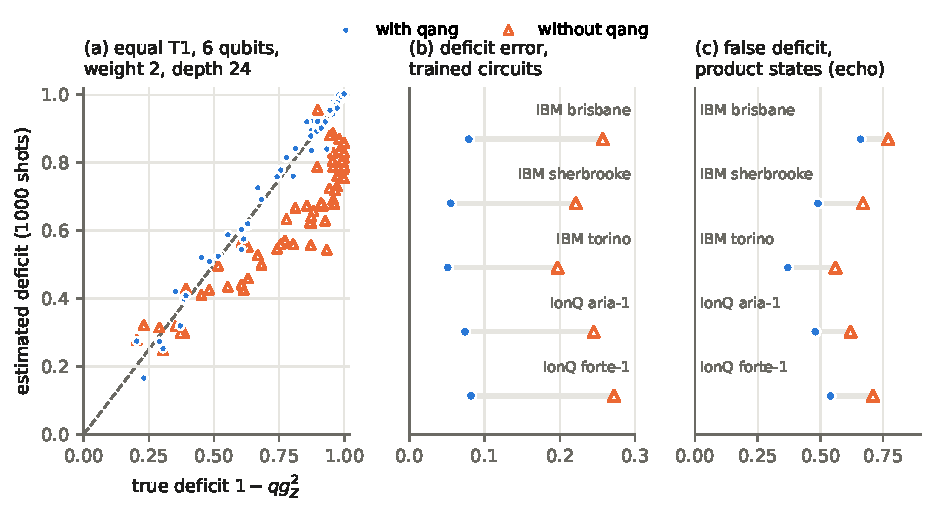
\includegraphics[width=\textwidth]{fig_radius.pdf}
\caption{(a) Estimated against true deficit, equal T1, 10 random circuits on 6 qubits, 1000 shots. (b) Mean absolute
error of the deficit on 30 trained circuits, five device noise models. (c) False deficit of the excited qubit of a
product state after an echo circuit (truth 0).}
\label{fig:main}
\end{figure}

\section{Device noise models}

A device adds gate errors, readout errors and time that a compiled two-qubit gate spends outside the weight sector,
where a decay can be rotated back in. We used the five-qubit weight-1 classifier of Ref.~\cite{monteverde2026qml}
compiled to Qiskit (19 RBS gates, 38--62 native two-qubit gates), on three IBM fake backends (Aer) and the IonQ cloud
simulator with the aria-1 and forte-1 noise models, 1000 shots. Trained circuits: 30 iris test inputs, true mean
deficit 0.37. Echo circuits: an excited basis state, the 15 trained gates and their inverse, truth 0. Four predictions
were committed before any noisy run (RESEARCH\_NOTES \S100).

\begin{table}[h]
\centering\small
\begin{tabular}{lcccc}
\toprule
backend & deficit error, trained & kept & false deficit, echo & two-qubit gates \\
 & with / without qang & shots & with / without qang & trained / echo \\
\midrule
IBM brisbane & 0.079 / 0.257 & 0.69 & 0.66 / 0.77 & 62 / 108 \\
IBM sherbrooke & 0.055 / 0.221 & 0.72 & 0.49 / 0.67 & 62 / 108 \\
IBM torino & 0.051 / 0.197 & 0.74 & 0.37 / 0.56 & 62 / 108 \\
IonQ aria-1 & 0.074 / 0.245 & 0.74 & 0.48 / 0.62 & 38 / 60 \\
IonQ forte-1 & 0.082 / 0.272 & 0.70 & 0.54 / 0.71 & 38 / 60 \\
\bottomrule
\end{tabular}
\caption{The radius deficit on device noise models (simulated, not hardware).}
\label{tab:dev}
\end{table}

On trained circuits the filtered deficit errs by 0.05--0.08, 3.2--4.0 times less than the unfiltered one
(Fig.~\ref{fig:main}b); three predictions passed on all five backends. The fourth failed on all five: we predicted
that the filter would remove more than half of the false deficit of a product state, and it removed 15--33\%
(Fig.~\ref{fig:main}c). The filter discards shots that left the sector, but errors that move the excitation inside
the sector pass it; here they affect 10--21\% of the kept shots on the excited qubit. Near a pole the deficit amplifies
them: a fraction $\varepsilon$ of misplaced shots reads as
\begin{equation}
D=4\varepsilon(1-\varepsilon),
\end{equation}
so 10\% already reads as 0.36. Where the true deficit is large the same errors change it little, which is why the
trained circuits fare well.

\section{Discussion}

The radius is a measure of entanglement only when the register is pure. Weight conservation and the qg filter make it
so exactly under one noise model, equal T1, and they do it from the Z-basis shots of the readout, with a shot cost
known in advance. On device noise the filtered radius remains a good estimate of a large deficit, but it is not a
reliable test of ``no entanglement'': in-sector errors, invisible to the filter, make product states look entangled.
A small deficit therefore needs a calibration, for example the echo circuit used here, or an error model.

\paragraph{What is new and what is not.} The radius, its relation to purity, the one-tangle and the Meyer--Wallach
measure are known~\cite{wootters1998,coffman2000,meyer2002,brennen2003}, and so is symmetry
verification~\cite{bonetmonroig2018,mcardle2019}. What we add is the combination: that in fixed-weight circuits the
radius is $|\qZ|$ and is read from Z-basis shots, that the filter makes it an entanglement measure under equal T1,
and measurements of how much of that survives unequal T1, dephasing and device noise models, with every prediction
committed before its run.

\paragraph{Limitations.} All noise is simulated, including the device noise models. The circuits are small (4--6
qubits). The echo circuits measure the false deficit of one family of product states. No quantum advantage is claimed.

\section*{Code and data availability}
Library \texttt{qang} 0.6.6 (MIT, \texttt{pip install qang}): \texttt{qang.formulation} (\texttt{radius\_profile},
\texttt{radius\_deficit}, \texttt{sphere\_area}, \texttt{meyer\_wallach}, \texttt{weight\_sector\_radius},
\texttt{gate\_radius\_class}, \texttt{algorithm\_radii}), \texttt{qang.statistics} (\texttt{qg2\_unbiased},
\texttt{radius2\_estimate}). Studies: \texttt{examples/qg\_radius\_witness\_qg.py} (\S98) and
\texttt{examples/qg\_radius\_hardware\_qg.py} (\S100), with predictions in their headers and tests in \texttt{tests/};
figure: \texttt{manuscript/radius/make\_figure.py}. Repository: \url{https://github.com/Viny2030/qang}.

\section*{Acknowledgments and use of AI tools}
Generative AI tools (Anthropic Claude Opus 5.5) assisted with code, numerical checks and drafting. The author proposed
the surface metric, framed the questions, and reviewed and validated all AI-assisted output.

\bibliographystyle{unsrtnat}
\bibliography{../refs}
\end{document}
